
\documentclass[11pt]{article}
\usepackage[a4paper,margin=1in]{geometry}
\usepackage[T1]{fontenc}
\usepackage[utf8]{inputenc}
\usepackage{lmodern}
\usepackage{microtype}
\usepackage{amsmath,amssymb,bm}
\usepackage{graphicx}
\usepackage{booktabs}
\usepackage{longtable}
\usepackage{array}
\usepackage{float}
\usepackage{caption}
\usepackage{setspace}
\usepackage{enumitem}
\usepackage{xcolor}
\usepackage{hyperref}
\hypersetup{colorlinks=true, linkcolor=black, citecolor=black, urlcolor=blue}
\setstretch{1.08}
\setlength{\parskip}{0.45em}
\setlength{\parindent}{1.0em}
\captionsetup{font=small,labelfont=bf}
\newcommand{\code}[1]{\texttt{#1}}
\newcommand{\riskbudget}{\varepsilon_{\mathrm{sev}}}

\title{\vspace{-1.5em}\textbf{Risk-Budgeted Information Release in Finite-Capacity Traffic Networks}\\[0.25em]
\large A Claim-Bounded Toy-Model Addendum to Socio-Traffic Thermodynamics}
\author{Keiji Yoshimura\\\small Independent Researcher}
\date{May 25, 2026\\[0.35em]\small Version: v0.3.0-synthesis-addendum\\\small Repository: \href{https://github.com/yokken0907/socio-traffic-thermodynamics}{github.com/yokken0907/socio-traffic-thermodynamics}}

\begin{document}
\maketitle

\begin{abstract}
This addendum extends Socio-Traffic Thermodynamics (STT) with a claim-bounded numerical synthesis focused on information release in finite-capacity traffic networks. The original STT manuscript framed congestion recurrence as a non-equilibrium dissipative pattern arising from density, delay, finite bandwidth, and social attraction. The present addendum narrows that framing to a tested toy-model question: when can route information reduce mean social cost without increasing overload severity relative to a conservative no-information baseline? Across STT v0.2.0--v0.2.9 toy audits, high-sensitivity, high-frequency, synchronous response to shared information repeatedly amplified overload, oscillation, and social cost. Conversely, low-rate, coarse, staggered, guarded, or otherwise risk-budgeted information release improved mean cost in the frozen holdout design while keeping overload severity at or below the no-information baseline. In the final v0.2.9 holdout, the best frozen policy, \code{budget\_common\_u0.055\_s0.00}, reduced mean cost from 1.758804 to 1.734372 and also reduced overload severity by 0.004088 relative to no information. The result should not be interpreted as a real-world traffic-control validation or as an argument for withholding information. It is a hypothesis-generating toy-model result: traffic information release should be treated as a risk-budgeted synchronization-control problem rather than a simple precision-maximization problem.
\end{abstract}

\section*{Reader Guidance and Claim Boundary}
This document is a toy-model synthesis addendum. It does not claim city-scale traffic prediction, policy validation, deployment readiness, route-guidance effectiveness, or a universal congestion solution. The allowed claim is narrower: within the tested finite-capacity toy networks and frozen holdout design, risk-budgeted low-rate/coarse/staggered information release reduced mean cost while not increasing overload severity relative to a no-information baseline.

The addendum is best read as a diagnostic bridge between classical traffic-flow instability, routing-game information effects, and a practical design question: how should information be released when a finite network can be destabilized by synchronized reactions?

\section{Background}
Traffic congestion can emerge endogenously without a fixed bottleneck in both car-following models and controlled experiments \cite{Bando1995,Sugiyama2008}. Broader traffic-flow theory has long treated vehicular traffic as a driven, many-particle, non-equilibrium system \cite{Helbing2001}. At the network level, selfish routing and information availability can also affect aggregate outcomes through equilibrium behavior, covariance of choices, and price-of-anarchy effects \cite{Roughgarden2003,Acemoglu2018}.

The original STT manuscript used this background to frame congestion as a recurrent dissipative structure on finite-bandwidth social-traffic networks. The present addendum does not expand that claim. Instead, it operationalizes one subclaim: route information can be harmful when it synchronizes reactions too strongly, and beneficial when its release is constrained by an explicit risk budget.

\section{Toy-Model Audit Program}
The v0.2.x program consisted of ten logged phases. Each phase preserved a toy-model claim boundary and avoided real-world policy interpretation.

\begin{longtable}{p{0.10\textwidth}p{0.50\textwidth}p{0.32\textwidth}}
\toprule
Phase & Purpose & Status \\
\midrule
\endhead
v020 & phase diagram and information-buffering preflight & PASS-STT-V020-PREFLIGHT-RAN \\
v021 & information-synchronization stress test & PASS-STT-V021-RUN-COMPLETE \\
v022 & desynchronization audit & PASS-STT-V022-RUN-COMPLETE \\
v023 & capacity-margin audit & PASS-STT-V023-RUN-COMPLETE \\
v024 & buffer-architecture audit & PASS-STT-V024-RUN-COMPLETE \\
v025 & mechanism-isolation audit & PASS-STT-V025-RUN-COMPLETE \\
v026 & topology and demand robustness audit & PASS-STT-V026-RUN-COMPLETE \\
v027 & risk-weighted Pareto audit & PASS-STT-V027-RUN-COMPLETE \\
v028 & risk-budgeted information release audit & PASS-STT-V028-RUN-COMPLETE \\
v029 & frozen-policy holdout audit & PASS-STT-V029-RUN-COMPLETE \\
\bottomrule
\end{longtable}

The final synthesis lock found all 10 phase outputs and 10 PASS-like phase statuses. The synthesis status was \code{PASS-STT-V030-SYNTHESIS-LOCKED}.

\section{Metrics and Risk-Budget Formulation}
Let $C$ denote mean social cost over a simulated condition, and let $S$ denote overload severity. The no-information policy is used as a conservative null baseline with metrics $(C_0,S_0)$. A candidate information policy $\pi$ is admissible under severity budget $\riskbudget$ if
\begin{equation}
S(\pi) - S_0 \leq \riskbudget.
\end{equation}
Among admissible policies, the toy-design objective is to reduce mean cost:
\begin{equation}
\Delta C(\pi) = C_0 - C(\pi) > 0.
\end{equation}
The strictest zero-budget condition is $\riskbudget=0$, meaning that the candidate must reduce mean cost without increasing overload severity relative to the no-information null.

This formulation deliberately separates average efficiency from overload risk. It also prevents the misleading conclusion that information should simply be maximized or withheld.

\section{Frozen Holdout Results}
The final v0.2.9 audit froze candidate policy families from the prior search and evaluated them on holdout topologies, pulse modes, utilizations, and seeds. Table~\ref{tab:policy_rollup} summarizes representative policy outcomes.

\begin{table}[H]
\centering
\small
\caption{Representative v0.2.9 frozen-holdout policy results. Positive improvement means lower mean cost than the no-information baseline.}
\label{tab:policy_rollup}
\resizebox{\textwidth}{!}{%
\begin{tabular}{llrrrr}
\toprule
Policy & Family & Mean cost & Overload severity & Sync index & Improvement \\
\midrule
budget\_common\_u0.055\_s0.00 & budget\_common & 1.734 & 0.0227 & 0.0028 & 0.024 \\
budget\_common\_u0.035\_s0.00 & budget\_common & 1.734 & 0.0228 & 0.0019 & 0.024 \\
coarse\_zone\_u0.035 & coarse\_zone & 1.736 & 0.0228 & 0.0041 & 0.023 \\
staggered\_private\_u0.035 & staggered\_private & 1.735 & 0.0228 & 0.0069 & 0.024 \\
no\_info & nan & 1.759 & 0.0268 & 0.0000 & 0.000 \\
common\_precise & common & 3.568 & 0.2177 & 0.9244 & -1.809 \\
delayed\_common & delayed & 6.716 & 0.4381 & 0.9391 & -4.957 \\
\bottomrule
\end{tabular}}
\end{table}

The best mean-cost frozen policy was \code{budget\_common\_u0.055\_s0.00}. Its mean cost was 1.734372 compared with 1.758804 for no information, giving an improvement of 0.024432. Its overload severity was 0.022745, which was 0.004088 lower than the no-information baseline. By contrast, \code{common\_precise} and \code{delayed\_common} substantially increased cost, overload severity, and synchronization index.

\begin{figure}[H]
\centering
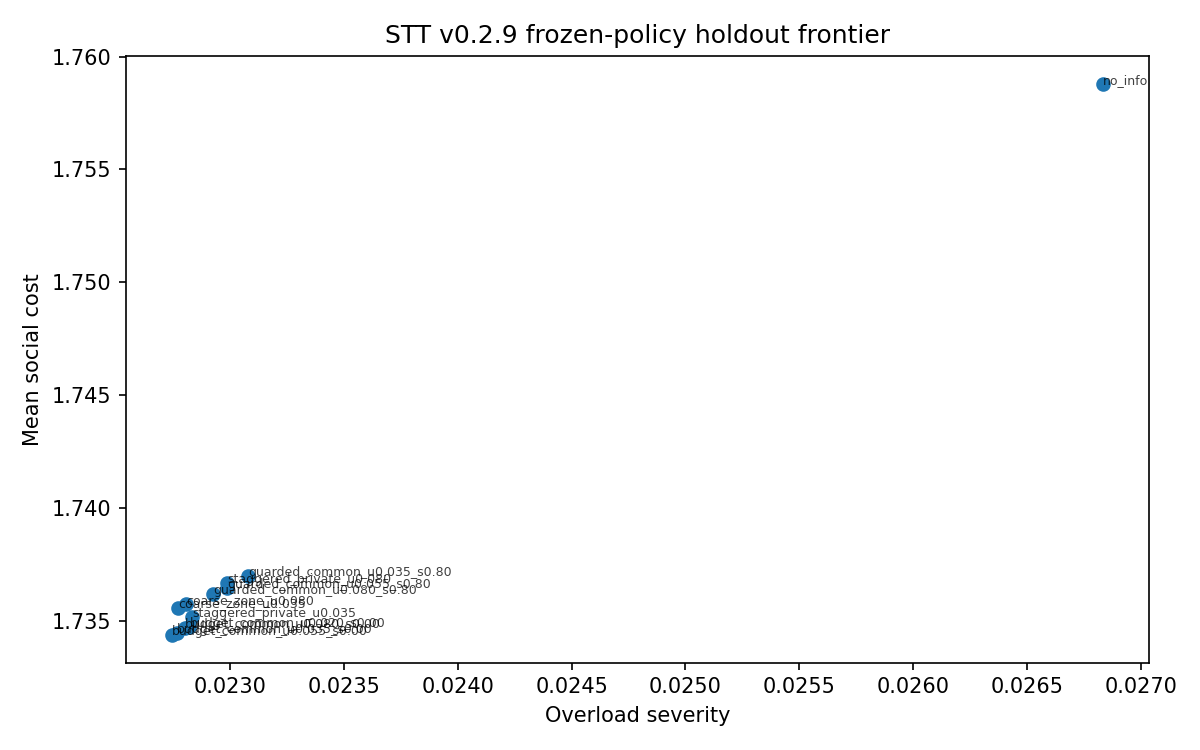
\includegraphics[width=0.88\textwidth]{figures/stt_v029_holdout_frontier.png}
\caption{Frozen-policy holdout frontier from STT v0.2.9. Candidate risk-budgeted policies lie close to the lower-left region, while the no-information baseline is more conservative but slightly less efficient.}
\label{fig:holdout_frontier}
\end{figure}

\section{Zero-Budget Finding}
Under the strict zero-budget condition, all 27 holdout conditions had at least one policy that improved mean cost without increasing overload severity relative to no information. The winning families were \code{budget\_common} and \code{coarse\_zone}.

\begin{table}[H]
\centering
\small
\caption{Zero-budget holdout winners.}
\label{tab:budget_winners}
\begin{tabular}{lrrrr}
\toprule
Winner family & Win count & Win fraction & Mean improvement & Mean sync index \\
\midrule
budget\_common & 20 & 0.741 & 0.0273 & 0.0039 \\
coarse\_zone & 7 & 0.259 & 0.0176 & 0.0040 \\
\bottomrule
\end{tabular}
\end{table}

The value curve in Figure~\ref{fig:budget_curve} is flat in the final holdout because zero-budget winners already existed in all holdout conditions. This is not a universal claim; it is a result of the tested candidate set and holdout design.

\begin{figure}[H]
\centering
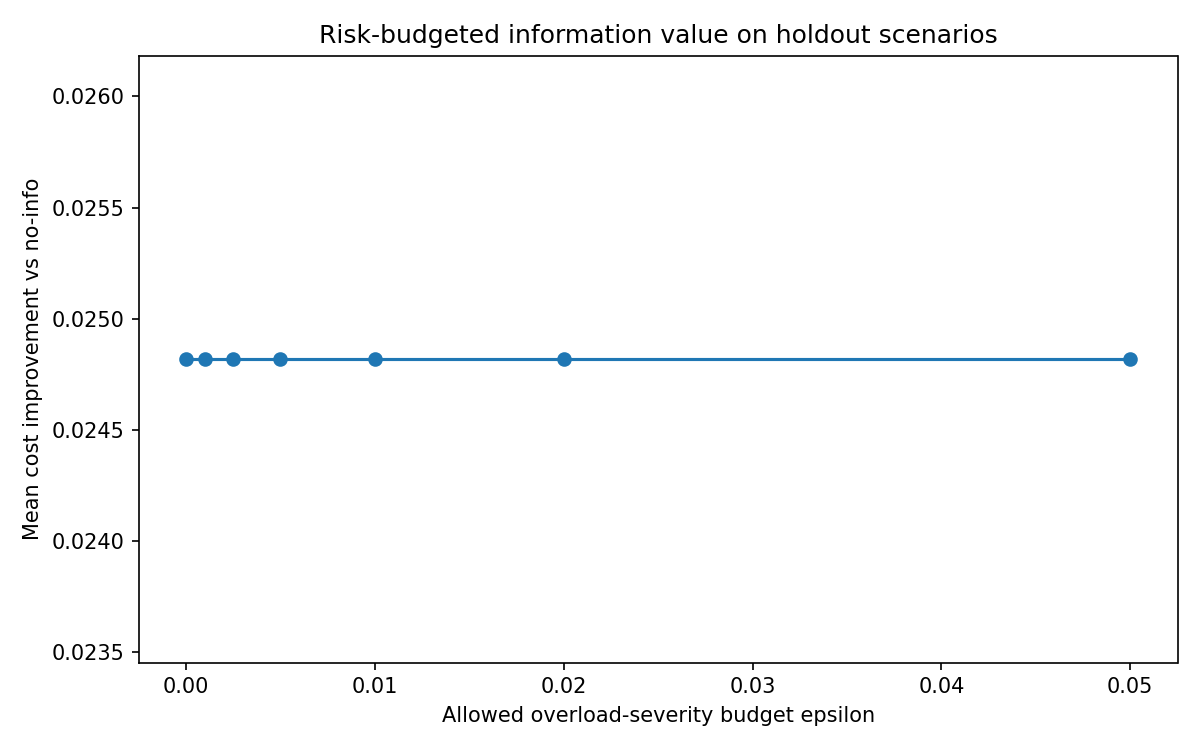
\includegraphics[width=0.88\textwidth]{figures/stt_v029_budget_value_curve.png}
\caption{Risk-budgeted information value in the frozen holdout. In this holdout, the best available candidate already improves mean cost at zero additional overload-severity budget.}
\label{fig:budget_curve}
\end{figure}

\section{Interpretation}
The main mechanism is not ``less information is always better.'' The observed mechanism is synchronization risk. Shared precise information can reduce individual uncertainty while increasing conditional action correlation. If many agents react in the same direction at the same time, finite-capacity links can be pushed into overload. Low-rate, coarse, staggered, or guarded release suppresses this action covariance and can preserve enough adaptation to improve mean cost.

This converts informational routing from a precision-maximization problem into a risk-budgeted release problem. A system designer must specify how much overload risk is acceptable, then choose a release rule that improves efficiency within that budget.

\section{Limitations}
The strongest limitation is model class. These are toy networks, not calibrated urban simulations. The policies are algorithmic abstractions rather than deployable route-guidance mechanisms. The metrics do not include equity, compliance heterogeneity, public trust, legal constraints, safety, multimodal behavior, or real sensor latency. Therefore, the result is a hypothesis-generating diagnostic claim rather than an operational traffic-policy claim.

A second limitation is that the no-information baseline is conservative in this toy design. Real traffic systems already contain heterogeneous information sources, institutional controls, learned behavior, and external routing platforms. Any empirical extension must define the baseline carefully.

\section{Next Validation Tier}
The appropriate next validation tier is not another small toy audit. The next step should use externally defined synthetic networks or public benchmark traffic scenarios with frozen candidate policies and predeclared metrics. The minimum extension should preserve: (i) a no-information or status-quo baseline, (ii) an overload-risk metric, (iii) a mean-efficiency metric, (iv) a synchronization metric, and (v) a frozen holdout protocol.

\section{Conclusion}
The v0.2.x STT audit program supports a narrower and stronger claim than the original broad framing. In finite-capacity toy networks, shared precise information can become harmful when it triggers high-frequency synchronized action. Risk-budgeted information release can reduce mean cost while respecting overload-risk constraints. The conceptual implication is that traffic information should be treated as a synchronization-control channel under finite capacity, not merely as a route-precision service.

\section*{Data and Code Availability}
This addendum is accompanied by the v0.3.0 synthesis package containing the synthesis report, claim lock, phase ledger, selected figures, and selected tables derived from the v0.2.0--v0.2.9 outputs. The original STT repository archive DOI 10.5281/zenodo.20201218 is retained as historical repository-archive context only. A new GitHub-Zenodo release, if created, should allow Zenodo to generate a new repository-archive DOI automatically.

\section*{Acknowledgments}
The author conceptually directed the theory-development and validation workflow. Large language models were used as computational, drafting, and software-assistance tools under direct human supervision. All claim-boundary decisions and release decisions remain the author's responsibility.

\begin{thebibliography}{99}
\bibitem{Bando1995}
M. Bando, K. Hasebe, A. Nakayama, A. Shibata, and Y. Sugiyama,
``Dynamical model of traffic congestion and numerical simulation,''
\emph{Physical Review E} \textbf{51}, 1035--1042 (1995). DOI: 10.1103/PhysRevE.51.1035.

\bibitem{Sugiyama2008}
Y. Sugiyama, M. Fukui, M. Kikuchi, K. Hasebe, A. Nakayama, K. Nishinari, S.-i. Tadaki, and S. Yukawa,
``Traffic jams without bottlenecks---experimental evidence for the physical mechanism of the formation of a jam,''
\emph{New Journal of Physics} \textbf{10}, 033001 (2008). DOI: 10.1088/1367-2630/10/3/033001.

\bibitem{Helbing2001}
D. Helbing,
``Traffic and related self-driven many-particle systems,''
\emph{Reviews of Modern Physics} \textbf{73}, 1067--1141 (2001). DOI: 10.1103/RevModPhys.73.1067.

\bibitem{Roughgarden2003}
T. Roughgarden,
``The price of anarchy is independent of the network topology,''
\emph{Journal of Computer and System Sciences} \textbf{67}(2), 341--364 (2003). DOI: 10.1016/S0022-0000(03)00044-8.

\bibitem{Acemoglu2018}
D. Acemoglu, A. Makhdoumi, A. Malekian, and A. Ozdaglar,
``Informational Braess' paradox: The effect of information on traffic congestion,''
\emph{Operations Research} \textbf{66}(4), 893--917 (2018). DOI: 10.1287/opre.2018.1719.

\bibitem{YoshimuraSTT2026}
K. Yoshimura,
\emph{Socio-Traffic Thermodynamics: Congestion as a Non-Equilibrium Dissipative Structure Driven by Social Potential},
repository archive, Zenodo (2026). DOI: 10.5281/zenodo.20201218.
\end{thebibliography}

\end{document}
